\section{RLC Netzwerke}
\subsection{Die Zeitkonstante Tau}
Die Zeitkonstante $\tau$ (Tau) beschreibt den Zusammenhang zwischen den verbauten Bauteilen. Somit können mithilfe von Spannungskurven auf die Bauteilwerte rückgeschlossen werden. \\
Eine weitere Möglichkeit auf Tau zu kommen ist die Berechnung mit den unten angegebenen Formeln:
\begin{itemize}
    \item RC-Netzwerk: {\large $\tau = R*C$}
    \item LR-Netzwerk: {\large $\tau = \frac{L}{R}$}
\end{itemize}
\subsubsection{Taumessung bei Ladekurven}
Tau kann sowohl beim Entladevorgang (siehe „Taumessung bei Entladekurven“) als auch beim Ladevorgang abgelesen werden. Bei Ladevorgängen wird eine Tangente aus dem Ursprung der Funktion gelegt. Diese Tangente schneidet anschließend den Maximalspannungswert. Wenn man diesen Schnittpunkt dann im 90° Winkel zur Zeitachse runter verbindet, kann Tau an diesem Punkt abgelesen werden:
\subsubsection*{RC-Glied}
\begin{center}
	\begin{circuitikz}
		\draw (0,0) to[R=$R$] (2,0);
		\draw (2,0) to[C=$C$] (2,-1.5);
		\draw (0,-1.5) -- (3,-1.5);
		\draw (2,0) -- (3,0);
		\draw[->,blue,>=latex,fill=blue] (0,-0.25) -- (0,-1.25) node[midway, left,blue] {${U}_e$};
		\draw[->,blue,>=latex,fill=blue] (3,-0.25) -- (3,-1.25) node[midway, right,blue] {${U}_a$};
		\draw[black,fill=black] (2,0) circle (1.5pt);
		\draw[black,fill=black] (2,-1.5) circle (1.5pt);
		\draw[black] (0,0) circle (1.5pt);
		\draw[black] (0,-1.5) circle (1.5pt);
		\draw[black] (3,0) circle (1.5pt);
		\draw[black] (3,-1.5) circle (1.5pt);
	\end{circuitikz}
\end{center}

\begin{center}
    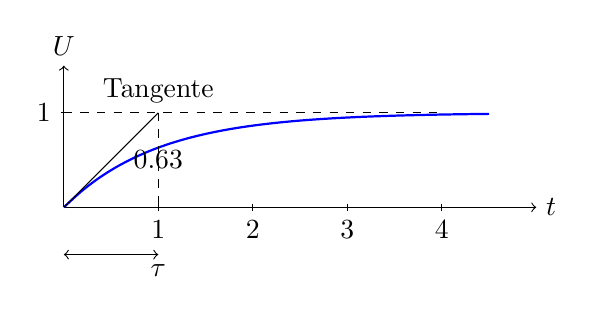
\begin{tikzpicture}[scale=1.2]
        % Achsen
        \draw[->] (0,0) -- (5,0) node[right] {$t$};
        \draw[->] (0,0) -- (0,1.5) node[above] {$U$};
        
        % Kurve
        \draw[thick, domain=0:4.5, smooth, variable=\x, blue] plot ({\x}, {1-exp(-\x)});
        
        % Beschriftungen
        \draw[dashed] (0,1) node[below] {} -- (4,1);
        \draw (0,0) -- (1,1) node[above] {Tangente};
        \draw[<->] (0,-0.5) -- (1,-0.5) node[below] {$\tau$};
        \draw[dashed] (1,1) -- (1,0) node[midway]{$0.63$};
        
        % Achsenbeschriftungen
        \foreach \x in {1,2,3,4}
            \draw (\x cm,1pt) -- (\x cm,-1pt) node[anchor=north] {$\x$};
        \foreach \y in {1}
            \draw (1pt,\y cm) -- (-1pt,\y cm) node[anchor=east] {$\y$};
            
    \end{tikzpicture}
\end{center}
Wichtige Kenndaten zu Tau bei Entladekurven:
\begin{itemize}
    \item Bei 63$\%$ der Maximalspannung kann Tau abgelesen werden.
    \item Bei 95$\%$ der Maximalspannung kann 2*Tau abgelesen werden.
    \item Bei 99$\%$ der Maximalspannung kann 3*Tau abgelesen werden
\end{itemize}
\subsubsection{Taumessung bei Entladekurven}
Im folgenden Bild ist die Spannung an einer Spule angegeben. Tau befindet sich bei 37$\%$ der Maximalspannung U0. Nach dem Einzeichnen der 37$\%$ kann $\tau$ auf der Zeitachse abgelesen werden:
%--------------------------
%   kommt noch was rein :3
%--------------------------
Wichtige Kenndaten zu Tau bei Entladekurven:
\begin{itemize}
    \item Bei 37$\%$ der Maximalspannung (nach 63$\%$ Abfall) kann Tau abgelesen werden.
    \item Bei 5$\%$ der Maximalspannung (nach 95$\%$ Abfall) kann 2*Tau abgelesen werden.
    \item Bei 1$\%$ der Maximalspannung (nach 99$\%$ Abfall) kann 3*Tau abgelesen werden.
\end{itemize}
\subsection{Schwingkreis}
Ein elektrischer Schwingkreis (auch als Resonanzkreis bekannt) ist eine resonanzfähige elektrische Schaltung aus einer Spule L und einem Kondensator C, die elektrische Schwingungen ausführen kann. In der Mechanik gibt es ebenfalls Schwingkreise. Diese sind aber für diese Mitschrift nicht von Bedeutung. Ein durchwegs bekanntes mechanisches Bauteil, welches elektrische Schwingungen erzeugen kann, ist der Quarz.

\subsubsection{LC-Schwingkreis}
Ein sogenannter LC-Schwingkreis besteht wie der Namen schon sagt aus einer Spule und einem Kondensator. Zusätzlich wird ein Widerstand eingebaut, dass der Schwingkreis ordentlich schwingen kann.
\begin{center}
	\begin{circuitikz}
        \draw (0,0) to[C=$C$] (0,-2);
        \draw (2,0) to[L=$L$] (2,-2);

        \draw (0,0) -- (2,0);
        \draw (0,-2) -- (2,-2);
	\end{circuitikz}
\end{center}
Um die Resonanzfrequenz oder auch umgangssprachlich Schwingfrequenz genannt, kann über die sogenannte „Thomsonsche Schwingungsformel“ berechnet werden:
\begin{center}
    \begin{Large}
    $f_{r} = \frac{1}{2 \cdot \pi \cdot \sqrt{L \cdot C}}$
    \end{Large}
\end{center}
Die Kreisfrequenz bei Resonanz wird mit der folgenden Formel berechnet:
\begin{center}
    \begin{Large}
    $\omega_{r} = \frac{1}{\sqrt{L \cdot C}}$
    \end{Large}
\end{center}
Die untere und die obere Grenzfrequenz ergeben sich aus den -3dB-Punkten (3dB-Bandgrenzen). Bei $\sqrt{2}$ der Maximalspannung können die Grenzfrequenzen berechnet werden. Ein anderer Weg auf die Bandgrenzen zu kommen ist es, drei dB von der Resonanzfrequenz abzuziehen und diese dann einzuzeichnen.
%--------------------------
%   kommt noch was rein :3
%--------------------------

\begin{center}
    \begin{Large}
    $B = f_{o} - f_{u}$     \\[10pt] 
    $B = \frac{f_{r}}{Q}$
    \end{Large}
\end{center}
\begin{itemize}
    \item B ... Bandbreite in Hz
    \item $f_{o}$ ... obere Grenzfrequenz in Hz
    \item $f_{u}$ ... untere Grenzfrequenz in Hz
    \item $f_{r}$ ... Resonanzfrequenz in Hz
    \item Q ... Güte des Resonanzkreises
\end{itemize}


\subsubsection*{Parallelschwingkreis}
\begin{center}
	\begin{circuitikz}
		\draw (3,-1) to[R=$R$] (3,-3);
		\draw (7,-1) to[C=$C$] (7,-3);
        \draw (5,0) to[L=$L$] (5,-4);

        \draw (0,0) -- (0,-1.5);
        \draw (0,-4) -- (0,-2.5);
        \draw (0,0) -- (5,0);
        \draw (0,-4) -- (5,-4);
        \draw (3,-1) -- (7,-1);
        \draw (3,-3) -- (7,-3);

        \draw[black] (0,-1.55) circle (2pt);
        \draw[black] (0,-2.45) circle (2pt);
		\draw[black,fill=black] (5,-1) circle (1.5pt);
		\draw[black,fill=black] (5,-3) circle (1.5pt); 

        \draw (-0.5,-2) .. controls (-0.25,-2.15) .. (0,-2);
        \draw (0,-2) .. controls (0.25,-1.85) .. (0.5,-2);

	\end{circuitikz}
\end{center}
\begin{center}
    \begin{Large}
    $Q = \frac{R}{X} = \frac{R}{2 \cdot \pi \cdot f_{r} \cdot L} =$ \\[10pt]
    $2 \cdot \pi \cdot f_{r} \cdot C \cdot R =$ \\[10pt]
    $R \cdot \sqrt{\frac{C}{L}} $
    \end{Large}
\end{center}
%--------------------------
%   kommt noch was rein :3
%--------------------------
Bei diesem Diagramm eilt die Spannung dem Strom hinterher.

\subsubsection*{Serienschwingkreis}
\begin{center}
\begin{circuitikz}
    \draw (0,0) to[R=$R$] (2,0);
    \draw (2,0) to[L=$L$] (4,0);
    \draw (4,0) to[C=$C$] (6,0);

    \draw (0,0) -- (0,-2);
    \draw (6,0) -- (6,-2);
    \draw (0,-2) -- (2.5,-2);
    \draw (6,-2) -- (3.5,-2);

    \draw[black] (2.57,-2) circle (2pt);
    \draw[black] (3.43,-2) circle (2pt);


    \draw (2.75,-2) .. controls (2.875,-2.15) .. (3,-2);
    \draw (3,-2) .. controls (3.125,-1.85) .. (3.25,-2);

\end{circuitikz}
\end{center}
\begin{center}
    \begin{Large}
    $Q = \frac{X}{R} = \frac{2 \cdot \pi \cdot f_{r} \cdot L}{R} =$ \\[10pt]
    $\frac{1}{2 \cdot \pi \cdot f_{r} \cdot C \cdot R}  =$ \\[10pt]
    $\frac{1}{R} \cdot \sqrt{\frac{L}{C}} $
    \end{Large}
\end{center}
%--------------------------
%   kommt noch was rein :3
%--------------------------
Bei diesem Diagramm eilt der Strom der Spannung hinterher.

\subsubsection{Quarz - Schwingkreis}
Hier angegeben ist der Pierce Oszillator. Dieser kann einfach mit einem Quarz der Wahl aufgebaut werden. Es kann durchaus möglich sein, dass es bei Microcontrollern oder ICs nötig ist, einen Quarzoszillator aufzubauen.
\begin{center}
	\begin{circuitikz}
		\draw (3,0) node[invschmitt]{} (4,0);
        \draw (1,0) node[american not port]{} (2,0);
		\draw (0,-2) to[R=$R1$] (2,-2);
        \draw (2,-2) to[R=$R2$] (2,-4);
		\draw (0,-4) to[C=$C1$] (0,-6);
        \draw (2,-4) to[C=$C2$] (2,-6);
        \draw (1,-4) node[piezoelectricshape]{} (2,-4);
        \draw (1,-6) node[rground]{};
        \draw (3.5,-2) node[rground]{};

        
        \draw (0,0) -- (0.5,0);
        \draw (0,0) -- (0,-4);
        \draw (0,-4) -- (0.7,-4);
        \draw (2,-4) -- (1.3,-4);
        \draw (2,0) -- (2,-2);
        \draw (0,-6) -- (2,-6);
        \draw (1.5,0) -- (2.5,0);
        \draw (3.5,-2) -- (3.7,-2);

        \draw[black] (3.8,0) circle (2pt);
        \draw[black] (3.8,-2) circle (2pt);
        \draw[black,fill=black] (2,0) circle (1.5pt);
        \draw[black,fill=black] (0,-2) circle (1.5pt);
        \draw[black,fill=black] (2,-2) circle (1.5pt);
		\draw[black,fill=black] (2,-4) circle (1.5pt);
		\draw[black,fill=black] (0,-4) circle (1.5pt);
        \draw[black,fill=black] (1,-6) circle (1.5pt);

		\draw[blue,>=latex,fill=blue] (4,-1.8) -- (4.4,-1.8);
		\draw[blue,>=latex,fill=blue] (4.4,-1.8) -- (4.4,-0.5);
		\draw[blue,>=latex,fill=blue] (4.4,-0.5) -- (4.8,-0.5);
		\draw[blue,>=latex,fill=blue] (4.8,-0.5) -- (4.8,-1.8);
		\draw[blue,>=latex,fill=blue] (4.8,-1.8) -- (5.2,-1.8);
		\draw[blue,>=latex,fill=blue] (5.2,-1.8) -- (5.2,-0.5);
        \draw[blue,>=latex,fill=blue] (5.2,-0.5) -- (5.6,-0.5);
        \draw[blue,>=latex,fill=blue] (5.6,-0.5) -- (5.6,-1.8);
		\draw[blue,>=latex,fill=blue] (5.6,-1.8) -- (6,-1.8);
        
	\end{circuitikz}
\end{center}
In dieser Schaltung wurden beispielsweise folgende Bauteilwerte genutzt:
\begin{itemize}
    \item $R_{1}: 100 k\Omega ... 10 M\Omega$
    \item $R_{2}: 10 \Omega ... 4.7 k\Omega$
    \item $C_{1}, C_{2}: 10 pF ... 82 pF$
\end{itemize}

\subsection{RLC-Kombinationen}
% \subsection{Tau-Messung}